%% Settings for single-side (simplex) printing
% Margins: left 40mm, right 25mm, top and bottom 25mm
% (but beware, LaTeX adds 1in implicitly)
\documentclass[12pt,a4paper]{report}
\setlength\textwidth{160mm}

\usepackage[utf8]{inputenc}
\usepackage{graphicx}
\usepackage{fancyhdr}
\usepackage{lmodern}
\usepackage{lastpage}
\usepackage{subfig}
\usepackage{hyperref}

\graphicspath{{../graphs/}}

\pagestyle{fancy}
\fancyhf{}
\rhead{Petr Houška `houskape@gmail.com`}
\lhead{HW3: Matrix transposition}
\rfoot{Page \thepage / \pageref{LastPage}}


\begin{document}
	
	\section{Reálné CPU}
	\begin{figure}[h]	
		\centering	
		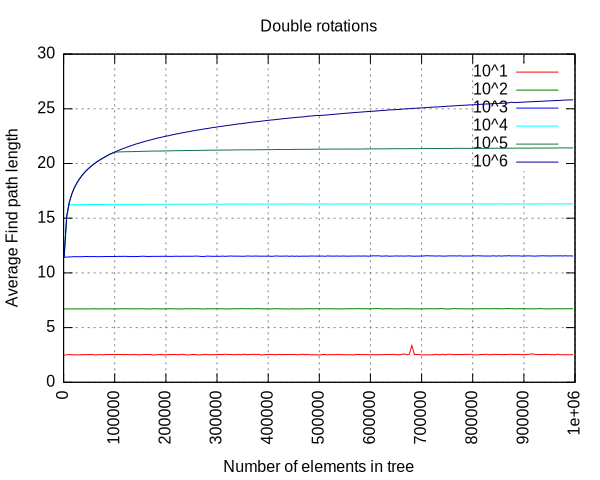
\includegraphics[scale=0.6]{graph_1}		
	\end{figure}

	Na prvním grafu vidíme porovnání průměrného času na prohození dvou prvků pro naivní algoritmus a rekurzivní cache oblivious algoritmus, který se zastaví na podmatici velikosti 8x8 a dál pokračuje naivně. 
	
	\subsection{Cache oblivious}
	
	Pro cache oblivious algoritmus jsou zřejmé dva segmenty, s rozhraním okolo cirka $800^2$ prvků. Skok mezi těmito dvěma segmenty není nikterak výrazný, z $1.5 * 10^{-6}$ na $4.0 * 10^{-6}$.
	
	Tento skok přibližně odpovídá tomu, kdy se celá matice ($640 000$ prvků, 3MB) ještě vleze do L3 cache. Skok tedy začíná trochu dříve než by čistě matematicky měl. I pro $n == 1000$ (4MB) by se do L3 matice měla vejít celá, nicméně kvůli asociativitě cache a komplikovanosti dnešního HW není úplně překvapivé, že ke zhoršování průměrného času dochází před úplným naplněním.
	
	Byť to z grafu není úplně vidět, tak čistá data naznačují, že podobný skok by mohl být i u hranice velikosti L2 a L3 cache. Konkrétně pro $n \approx 256$, kdy se celá matice ještě vejde do L2, se průměrný čas přístupu zvedne z $1.2 * 10^{-6}$ na $1.4 * 10^{-6}$. Kvůli šumu a skokům k vyšším hodnotám pro určitá $n$ (téměř jistě kvůli asociativitě) se ovšem nedá říct nic s jistotou. 
	
	Na rozhraní $n$ pro matice, které se těsně vejdou do L1 cache žádný pozorovatelný rozdíl není. 
			
	\subsection{Naive}
	U naivního algoritmu jsou jasně pozorovatelné segmenty 3. Od začátku do $1000^2$ prvků, kde se průměrný čas pohybuje okolo $1.5 * 10^{-6}$, tedy stejně jako u cache oblivious algoritmu. Následně do 	$20 000^2$ prvků, kdy je čas okolo $1-2 * 10^{-5}$, a nakonec poslední segment, ve kterém čas roste až k $5*10^{-5}$ milisekund na prohození.
	
	
	První skok odpovídá již dříve popsanému přechodu z toho, kdy se celá matice ještě vleze do L3 cache a kdy už ne. Dokud se vleze, tak je naivní algoritmus, s výjimkou $n == 512$, naprosto srovnatelný s cache aware variantou. Pro $n == 512$ se téměř určitě projevuje asociativita cache. Ta má která má, vzhledem k access patternu, daleko větší dopad v případě naivního přístupu (kde přistupujeme postupě na všechny řádky pod sebou, které jsou od sebe přesně o $4*512$B) než v případě cache oblivious.
	
	To že je naivní přístup až do $n$, kdy se matice nevejde do L3 cache, srovnatelný s cache oblivious algoritmem jen dále podporuje tezi, že mezi tím, jestli se matice vejde do L1, L2 nebo jen L3 není žádný významně pozorovatelný rozdíl, který by nebyl z větší části vynahrazen cache pre-fetchem a zamaskován ostatními vlivy. Pokud by totiž přesouvání z L3 cache do L1 a L2 mělo výrazný overhead, tak by se tento overhead nutně více projevil v naivním algoritmu (cache oblivious přístup tyto přesuny minimalizuje).
	
	Od $n$, kdy se matice už nevleze do L3 cache roste průměrná doba swapu postupně až do $n \approx 22 000$ (matice velikosti 2GB), kdy začne raketově růst z $2 * 10^{-5}$ k $5 * 10^{-5}$ milisekundám. Tam se následně, byť v velkým rozptylem, drží až do maximální testované velikostí $n == 44591$ (7.9 GB).
	
	Tento růst a obecně velký rozptyl v druhém i třetím segmentu si vysvětlují tím, jak je paměť RAM strukturovaná. Za zmínku stojí ještě vyšší průměrný čas vždy když je $n$ násobkem mocin $2$. Z části to bude způsobené tím, že u poloviny přístupů (ty co jdou v rámci řádku) se bude více projevovat cache aliasing (viz výše) způsobený asociativností cache. Z části to může být způsobené také strukturou paměti RAM, nicméně na posouzení toho co má konkrétně jaký vliv nemám dostatečné znalosti.
	
	\section{Simulátor}
	\begin{figure}[h]	
	\centering	
	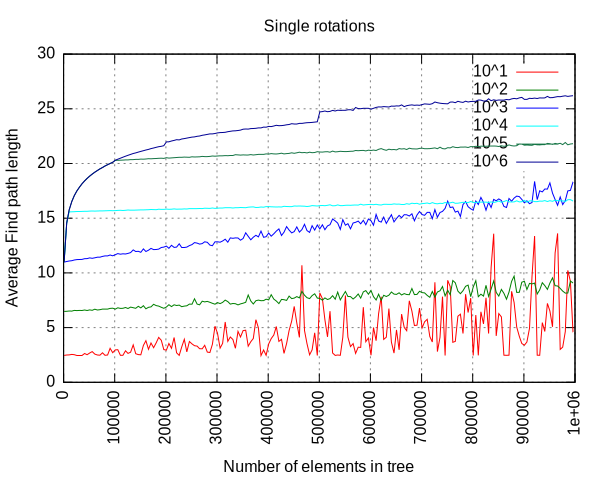
\includegraphics[scale=0.6]{graph_2}		
	\end{figure}

	Na grafu ze simulátoru je hned na první pohled pozorovatelný jeden fakt. Zatímco cache oblivious algoritmus drží průměrný počet načtených bloků vůči velikosti matice (nebo jejího řádku) konstnatní, tak pro naivní začne vždy od nějakého $n$ průměrný počet načtených bloků růst k číslu okolo $1$. To odpovídá tomu, že jeden ze dvou přístupů swapu (ten co jde ve sloupci) způsobí vždy načtení nového bloku.
	
	Naopak pro cache oblivious přístup je zjevná periodicita. Pro $n$ mocniny dvojky je průměrný počet načtených bloků vždy nižší než pro ostatní $n$. To je způsobeno tím, že pro $n$ mocniny dvojky jsou všechny rekurzivní podmatice vždy zarovnané na začátky cache řádků tím nejlepším způsobem, jak jen mohou být.
	
	\subsection{Naivní přístup}
	
	\begin{figure}[h]	
		\centering	
		\includegraphics[scale=0.6]{graph_2_naive}		
	\end{figure}
	
	Jak bylo řečeno již výše, tak v naivním přístupu pro každou konfiguraci cachí platí následující. Průměrný počet načtených bloků je konstantní až do velikosti, kdy má matice více řádků než kolik má cache bloků, v ten moment začne růst k 1. Zlomová velikost vždy odpovídá tomu, kdy začne mít matice více řádků než kolik je cache bloků. 
	
	Jakmile má totiž matice více řádků než je cache bloků, tak naivní přístup z cache vyhodí v rámci přístupů po řádcích kvůli $radku > cacheBloku$ první řádek. A v rámci dalšího průchodu tak první řádek musí znovu načíst. To ale vyhodí druhý řádek, a tak dále. Přístup po řádcích tedy vždy vyústí v načtení jednoho bloku.
	
	Tento efekt se nezačne projevovat úplně ostře (zlom není ostrý z malých hodnot rovnou k 1) kvůli tomu, že počet efektivních řádků z pohledu algoritmu se lineárně mění z 1 do $n$. U přístupů v rámci řádků totiž jedeme v horním trojúhelníku (nad diagonálou) a u přístupů po řádcích v dolním trojúhelníku (pod diagonálou). Díky tomu po zlomu roste průměrný počet načtených bloků postupně (v relaci k tomu jakou část běhu algoritmu je počet řádků větší než počet bloků cache). Čím je počet bloků větší tím postupnější je tento přechod.

	Pro přístupy v rámci řádku (v naivním algoritmu je vždy jedne po řádcích a jeden v rámci řádku) se pak s $n$ nic nemění. Konfigurace cache jen ovlivňuje, jaký je průměrný počet načtených bloků na jeden přístup. Různost těchto čísel pro různé konfigurace způsobuje, proč po zlomovém bodě nekonvergují všechny průměrné počty přístupů k jendomu číslu, ale proč jdou konfigurace s delšími cache bloky k $1$ a ty s kratšími jdou k hodnotě $> 1$. Konkrétně pro cache bloky o 64B k $1 + 1/(64 / 4) = 1.062$
		
	Co se týče průběhu před zlomem, tak tam se výše popsaný průměrný počet bloků na přístup v rámci řádku projevuje také, což vysvětluje různé výšky ze začátku. Například pro konfiguraci 64x1024 a 64x4096 je to $2 * 1.062 = 0.124$. Načtení nového bloku je totiž třeba každých $64 / 4$ bloků pro přístupy v rámci řádku a to samé v rámci sloupců (každých $64 / 4$ sloupců je potřeba načíst pro každý prvek ve sloupci, pro zbylé sloupce se jede z již načtených bloků). Obdobně pro ostatní konfigurace.


	\subsection{Cache oblivious přístup}
	
	\begin{figure}[h]	
		\centering	
		\includegraphics[scale=0.6]{graph_2_adv}		
	\end{figure}
	
	Předně, pro všechny konfigurace platí, že dokud se celá matice vejde do cache, tak je průměrný počet bloků víceméně konstantní. Nepřekvapivě odpovídající přibližně $1\over(velikostCache/4)$. 
	
	Jakmile je tento počet překročen tak začne průměrný počet bloků stoupat. Pro konfigurace, které mají cache bloky v tomto bodě menší než $n$ (první tři), přejde do periodického  stavu, který odpovídá ideálnímu chování z přednášky. Tedy takovému, kdy se matice rekurzí rozdělí na právě takové podmatice, aby se právě vešly do cache. 
	
	Zde je také krásně pozorovatelné, že pro mocniny se tento periodický stav přibliží - v průměrném počtu načtených bloků - ideálnímu stavu, kdy se celá matice vešla do cache. Všechny rekurzivní podmatice jsou totiž při $n = 2^k$ dokonale zarovnané, jednotlivé cache bloky pro rekurzivní volání se tedy nepřekrývají a situace je ideální.
	
	Pro $n != 2^k$ je pak vždy pozorovatelný horší průměrný počet načtených bloků. Čím je cache méně, tj. do čím menších podmatic se rekurze musí dostat než se vše vejde do cache, tím jsou hodnoty pro nemocniny dvojky horší. Tím větší podíl totiž mají ony okrajové bloky, které se překrývají s okolními rekurzivními podmaticemi kvůli nedokonalému zarovnání adres, a které tedy musí být načtené vicekrát.
	
	Další jev, který si zaslouží zmínit je pozvolný nástup pro konfiguraci 4096x64 a do menší míry i 512x512. Ten je způsoben tím, že pro menší $n$ je řádek matice kratší než blok cache, jeden přístup tedy způsobí načtení hned několika řádků.
	
	Poslední úkaz, který si zaslouží zmínit je relativní velikost čísel pro jednotlivé konfigurace. Zatímco první tři konfigurace mají výrazně rozdílné absolutní velikosti cache tak sdílí base-line úroveň pro ideální využítí cache (u $n == 2^k$). To je způsobeno tím, že kvůli tomu, že mají stejně velký cache blok, tak i v ideálním případě musí každých $64$-čtení dojít k načtení nového bloku.
	
	Naopak s větším cache blokem, i když celková velikost cache není větší, může být počet čtení teoreticky výrazně menší. Jediné místo, kde by to nemusela být pravda je konfigurace 4096x64 neb u ní není zaručeno, že si řádek nevyhodíme (výrazně) dřív než budeme moci jeho zbytek použít. To je také důvodem, proč je tato konfigurace horší než 512x512. Díky tomu, jak jsem implementoval metodu `TransposeAndSwitch` jde ovšem rekurze po podmaticích vedle sebe a je tedy schopná efektivně pracovat na dvou podmaticích 32x32 vedle sebe v cache než si načtené bloky vyhodí. To je důvod, proč je lepší než konfigurace 64xYY, které jsou schopné efektivně pracovat jen s aktuální jednou podmaticí 32x32 v cache.

\end{document}